\section{Methods}
\label{sec:methods}

All models were written from scratch in PyTorch and trained with one shared training loop, so that differences between models come from the architecture or strategy and not from the training recipe (\cref{fig:design}).

\begin{figure}[t]
\centering
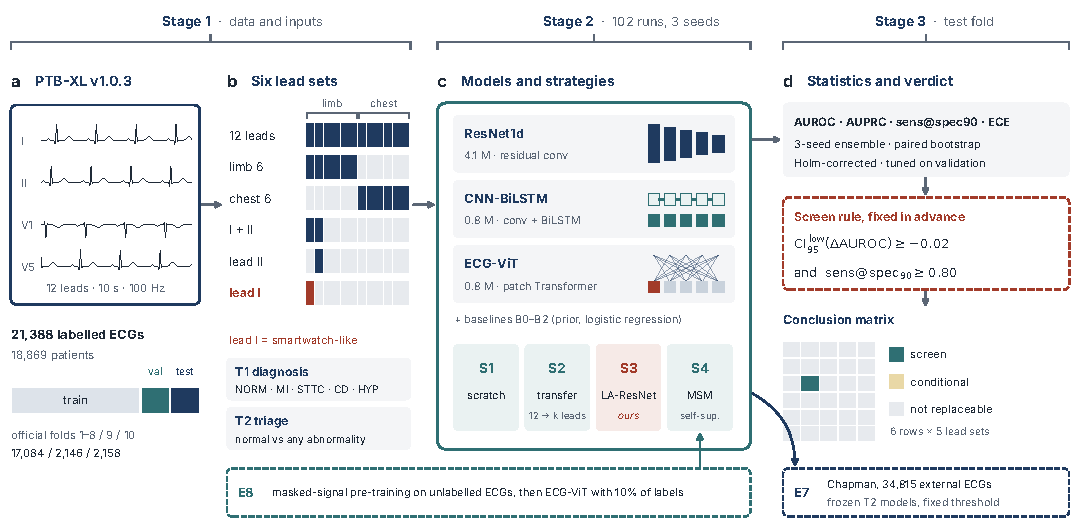
\includegraphics[width=\linewidth]{figA_study_design.pdf}
\caption{Study design. \textbf{a}, PTB-XL records and the official patient-level folds. \textbf{b}, six lead configurations, from 12 leads to the smartwatch-like lead I, each trained and tested separately, for diagnosis (T1) and triage (T2). \textbf{c}, three architectures with different inductive biases and four training strategies (S3 is our lead-agnostic model), plus baselines B0--B2; 102 runs with three seeds. \textbf{d}, test-fold statistics, the screen rule fixed before any result, and the resulting conclusion matrix. Dashed boxes: self-supervised pre-training with 10\% labels (E8) and external validation of frozen models on 34,815 Chapman ECGs (E7), which reports external metrics only.}
\label{fig:design}
\end{figure}

\subsection{Baselines}
\begin{itemize}
  \item \textbf{B0 (prior)} predicts each class's training prevalence for every record (AUROC $=0.5$ by construction).
  \item \textbf{B1 (pre-specified)} is a logistic regression ($C=0.1$) on the standardised signal after $4\times$ average pooling (3,000 features for 12 leads).
  \item \textbf{B2 (feature baseline).} B1 performed at chance (\cref{sec:res_arch}) because a fixed time sample means different things in different records: beats are not aligned across recordings. B2 therefore summarises each lead with 22 shift-invariant features (13 amplitude statistics, 2 slope statistics, relative power in 5 frequency bands, and the dominant autocorrelation period and its strength as a rhythm estimate) and fits the same logistic regression. B2 was added after B1 failed; B1 is kept and reported unchanged.
\end{itemize}

\subsection{Architectures: three inductive biases}
\begin{itemize}
  \item \textbf{ResNet1d} (4.07\,M parameters) is a one-dimensional residual network~\cite{he2016resnet}: a stride-2 convolution (kernel 15) and max-pooling stem, eight basic residual blocks (kernel 7) widening from 64 to 256 channels in three stride-2 stages, concatenated global average and max pooling, dropout 0.2 and a linear head. Its receptive field is 1,291 samples, longer than the 10\,s input. \emph{Bias:} local, translation-equivariant morphology detectors stacked hierarchically.
  \item \textbf{CNN-BiLSTM} (0.79\,M) combines a convolutional stem that down-samples by 4 (250 time steps), a two-layer bidirectional LSTM~\cite{hochreiter1997lstm} (hidden size 128, dropout 0.3) and additive attention pooling over time. \emph{Bias:} local feature extraction followed by sequential modelling of beat-to-beat context.
  \item \textbf{ECG-ViT} (0.82\,M) is a one-dimensional Vision Transformer~\cite{dosovitskiy2021vit}. The recording is split into 50 non-overlapping 200\,ms patches (20 samples $\times$ all leads), linearly embedded ($D=128$), prefixed with a learnable CLS token and summed with a sinusoidal position encoding, then passed through four pre-LayerNorm Transformer blocks~\cite{vaswani2017attention} (four heads, MLP width 512) with hand-written multi-head self-attention; the CLS token feeds the classifier. \emph{Bias:} weak locality prior, global interactions between all patches from the first layer.
\end{itemize}

\subsection{Training strategies}
\begin{itemize}
  \item \textbf{S1 -- from scratch:} one model per lead configuration.
  \item \textbf{S2 -- supervised transfer} starts from the 12-lead ResNet1d of the same seed. The first convolution is replaced by one with the reduced number of input leads, and the 12-lead filters of the leads that remain are copied into it. \emph{Fine-tune:} all layers are trained, the new input layer and head at the base learning rate and the backbone at $0.1\times$ (discriminative learning rate). \emph{Frozen:} only the new input layer and the head are trained (lead I only).
  \item \textbf{S3 -- LA-ResNet (lead-agnostic; our design)} is one ResNet1d with 24 input channels: the 12 standardised leads, with missing leads set to zero, plus 12 constant 0/1 mask channels that tell the network which leads are real. During training each record is shown with all 12 leads (probability 0.5), one of the five reduced configurations (0.3) or a random lead subset (0.2). Early stopping uses the mean validation AUROC over all six configurations, so a single checkpoint serves every configuration at test time.
  \item \textbf{S4 -- self-supervised pre-training (E8).} ECG-ViT is first trained without labels by masked signal modelling, following the masked-modelling idea of BERT and masked autoencoders~\cite{devlin2019bert,he2022mae}: 8 of the 50 patches ($\approx$15\%) are replaced by a learnable mask embedding and the network reconstructs their standardised samples (mean squared error on the hidden patches only). Pre-training used all training-fold records without labels (one encoder for 12lead and one for leadI; up to 100 epochs; early stopping on the validation reconstruction error). The encoder was then fine-tuned with a new classification head on 10\% of the training patients' labels, with all layers at the same learning rate as S1.
\end{itemize}

\subsection{Shared training recipe}
All supervised models used binary cross-entropy with logits, AdamW~\cite{loshchilov2019adamw} (learning rate $10^{-3}$, weight decay $10^{-2}$), a one-cycle learning-rate schedule~\cite{smith2019onecycle} with 10\% warm-up, batch size 128, gradient-norm clipping at 1.0 and mixed precision on the GPU. Training ran for at most 50 epochs with early stopping on validation macro AUROC (patience 10); the best weights were kept as a deep copy and restored. Training-time augmentation consisted of per-lead amplitude scaling ($\sigma=0.1$), a baseline offset ($\sigma=0.05$), additive Gaussian noise ($\sigma=0.02$) and a random circular shift of up to $\pm0.5$\,s. No hyper-parameter was tuned for any individual model. Every configuration in the main grid was trained with three seeds (0, 1, 2), except the ablations and label-efficiency runs, which used seed 0 as pre-specified.

\subsection{Experiments}
\Cref{tab:experiments} lists the experiment grid: 102 supervised runs in the main grid and 14 runs in E8. Subsets of training patients in E5 and E8 were drawn per seed at the patient level, and both arms of E8 used the same subset within a seed.

\begin{table}[H]
\centering
\small
\caption{Experiment grid.}
\label{tab:experiments}
\begin{tabular}{lp{7.2cm}p{5.2cm}}
\toprule
ID & Question & Runs \\
\midrule
E0 & Baselines B0--B2 (12lead, leadI; T1, T2) & CPU only \\
E1 & Architectures on 12 leads & 3 models $\times$ 3 seeds = 9 \\
E1b & Ablations: no residual; kernel 3/15/31; vanilla RNN; class-weighted loss & 6 (seed 0) \\
E2 & Reduced leads, trained from scratch & 3 models $\times$ 5 configurations $\times$ 3 seeds = 45 \\
E3 & Training strategies & S2 fine-tune 15 + S2 frozen 3 + S3 3 = 21 \\
E4 & T2 triage & ResNet1d $\times$ \{12lead, leadI\} $\times$ 3 + LA-ResNet $\times$ 3 = 9 \\
E5 & Label efficiency (10/25/50\% of training patients) & 12 (seed 0) \\
E7 & External validation (frozen models) & 0 \\
E8 & Self-supervised pre-training & 2 pre-training + 12 fine-tuning \\
\bottomrule
\end{tabular}
\end{table}
